\documentclass[aspectratio=169, 10pt]{beamer}

\usetheme{Madrid}
\usecolortheme{seahorse}
\usefonttheme{professionalfonts}

\usepackage{booktabs}
\usepackage{amsmath}
\usepackage{graphicx}
\usepackage{xcolor}
\usepackage{tikz}
\usepackage{pgfplots}
\usepackage{pgfplotstable}
\usepackage{colortbl}
\usepackage{multirow}

\pgfplotsset{compat=1.17}
\usetikzlibrary{arrows.meta, shapes.geometric, positioning, fit, backgrounds, decorations.pathreplacing, calc}

% ── Colours ──────────────────────────────────────────────────────────────────
\definecolor{accent}{RGB}{0, 90, 156}
\definecolor{good}{RGB}{34, 139, 34}
\definecolor{bad}{RGB}{180, 30, 30}
\definecolor{blockbg}{RGB}{230, 240, 255}
\definecolor{cspblue}{RGB}{173, 216, 230}
\definecolor{neckyellow}{RGB}{255, 223, 128}
\definecolor{headgreen}{RGB}{144, 238, 144}
\definecolor{lossred}{RGB}{255, 182, 193}
\definecolor{rowhl}{RGB}{220, 235, 255}

\setbeamercolor{frametitle}{bg=accent, fg=white}
\setbeamercolor{title}{fg=accent}
\setbeamercolor{structure}{fg=accent}

% ─────────────────────────────────────────────────────────────────────────────
\title[Ultrasound Object Detection]{Object Detection in Ultrasound\\{\large Model Development Summary}}
\subtitle{PP-YOLOE with Ultrasound-Specific Adaptations}
\author{Dhanesh Ramachandram}
\date{\today}

% ─────────────────────────────────────────────────────────────────────────────
\begin{document}

\begin{frame}
  \titlepage
\end{frame}

% ── AGENDA ───────────────────────────────────────────────────────────────────
\begin{frame}{Agenda}
  \tableofcontents
\end{frame}

\section{Architecture \& Setup}
\section{Loss Functions}
\section{Training Stability Fixes}
\section{Data \& Augmentation}
\section{Metrics \& Reproducibility}
\section{Hyperparameter Optimisation}
\section{Baseline vs PU Loss — Full Training Comparison}

% ── SLIDE 2 — Architecture ───────────────────────────────────────────────────
\begin{frame}{Model Architecture — PP-YOLOE}
  \begin{columns}[T]
    \begin{column}{0.55\textwidth}
      % TikZ architecture diagram
      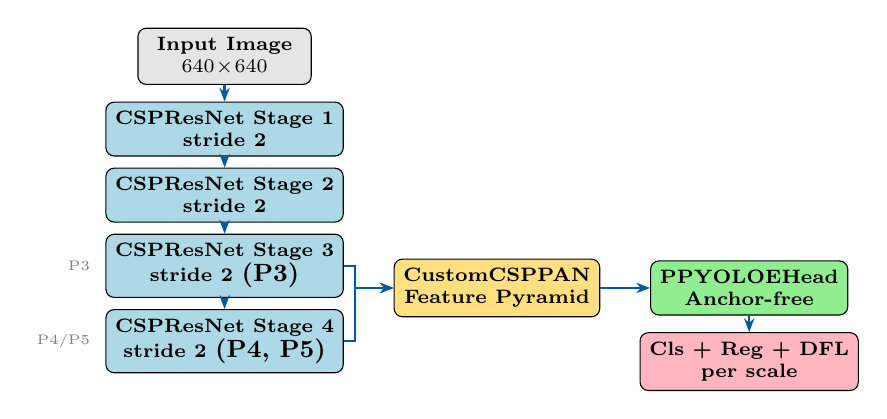
\begin{tikzpicture}[
          node distance=4pt,
          box/.style={draw, rounded corners=3pt, minimum width=2.2cm, minimum height=0.55cm,
                      font=\scriptsize\bfseries, align=center},
          arr/.style={-{Stealth[length=5pt]}, thick, color=accent},
          lbl/.style={font=\tiny, color=gray}
        ]
        % Input
        \node[box, fill=gray!20] (inp) {Input Image\\$640\!\times\!640$};
        % Backbone stages
        \node[box, fill=cspblue, below=6pt of inp] (b1) {CSPResNet Stage 1\\stride 2};
        \node[box, fill=cspblue, below=4pt of b1]  (b2) {CSPResNet Stage 2\\stride 2};
        \node[box, fill=cspblue, below=4pt of b2]  (b3) {CSPResNet Stage 3\\stride 2 \small(P3)};
        \node[box, fill=cspblue, below=4pt of b3]  (b4) {CSPResNet Stage 4\\stride 2 \small(P4, P5)};
        % Neck
        \node[box, fill=neckyellow, right=18pt of b3, yshift=-8pt] (neck) {CustomCSPPAN\\Feature Pyramid};
        % Head
        \node[box, fill=headgreen, right=18pt of neck, yshift=0pt] (head) {PPYOLOEHead\\Anchor-free};
        % Outputs
        \node[box, fill=lossred, below=6pt of head] (out1) {Cls + Reg + DFL\\per scale};

        \draw[arr] (inp) -- (b1);
        \draw[arr] (b1)  -- (b2);
        \draw[arr] (b2)  -- (b3);
        \draw[arr] (b3)  -- (b4);
        \draw[arr] (b3.east) -- ++(4pt,0) |- (neck.west);
        \draw[arr] (b4.east) -- ++(4pt,0) |- (neck.west);
        \draw[arr] (neck) -- (head);
        \draw[arr] (head) -- (out1);

        % Labels
        \node[lbl, left=2pt of b3] {P3};
        \node[lbl, left=2pt of b4] {P4/P5};
      \end{tikzpicture}
    \end{column}
    \begin{column}{0.42\textwidth}
      \vspace{4pt}
      \begin{block}{Component summary}
        \small
        \begin{tabular}{ll}
          \toprule
          Component & Role \\
          \midrule
          CSPResNet   & Multi-scale features \\
          CSPPAN      & Feature pyramid fusion \\
          PPYOLOEHead & Task-aligned, anchor-free \\
          ATSSAssigner & Dynamic target assignment \\
          DFL ($\text{reg\_max}=16$) & Uncertainty-aware boxes \\
          \bottomrule
        \end{tabular}
      \end{block}
      \vspace{4pt}
      \textbf{Why anchor-free?} No grid tuning needed for variable lesion sizes in ultrasound.\\[4pt]
      \textbf{Why DFL?} Soft US boundaries $\Rightarrow$ box uncertainty matters.
    \end{column}
  \end{columns}
\end{frame}

% ── SLIDE 3 — Loss Functions ─────────────────────────────────────────────────
\begin{frame}{Loss Functions}
  \begin{columns}[T]
    \begin{column}{0.50\textwidth}
      \textbf{Baseline \texttt{YOLOELoss}}
      \[
        \mathcal{L} = \mathcal{L}_{\text{cls}} + \mathcal{L}_{\text{reg}} + \mathcal{L}_{\text{DFL}}
      \]
      \vspace{-6pt}

      % Loss normalisation comparison table
      \begin{center}
      {\tiny
      \begin{tabular}{lll}
        \toprule
        & \textbf{Before (buggy)} & \textbf{After (fixed)} \\
        \midrule
        Pos cls & \texttt{.mean() * w} & \texttt{.sum() / num\_pos} \\
        Neg cls & \texttt{.mean()}      & \texttt{.sum() / num\_pos} \\
        Imbalance & $\sim$30,000$\times$ & balanced \\
        Precision & 1--3\%              & {\color{good}40--52\%} \\
        \bottomrule
      \end{tabular}
      }
      \end{center}

      \vspace{2pt}
      Label smoothing: positive targets $\to 1-\epsilon$, $\epsilon=0.1$
    \end{column}
    \begin{column}{0.46\textwidth}
      \textbf{PU-Loss \texttt{YOLOEPUFocalLoss}}\\[3pt]
      {\small For $\sim$10\% labeled data scenarios:}

      \vspace{4pt}
      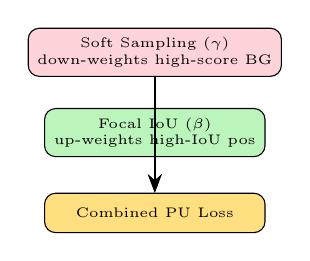
\begin{tikzpicture}[scale=0.85, every node/.style={font=\tiny}]
        \node[draw, fill=lossred!60,   rounded corners, minimum width=2.8cm, minimum height=0.5cm, align=center] (sg) at (0,1.2) {Soft Sampling ($\gamma$)\\down-weights high-score BG};
        \node[draw, fill=headgreen!60, rounded corners, minimum width=2.8cm, minimum height=0.5cm, align=center] (fi) at (0,0)   {Focal IoU ($\beta$)\\up-weights high-IoU pos};
        \node[draw, fill=neckyellow,   rounded corners, minimum width=2.8cm, minimum height=0.5cm, align=center] (cl) at (0,-1.2){Combined PU Loss};
        \draw[-{Stealth}, thick] (sg) -- (cl);
        \draw[-{Stealth}, thick] (fi) -- (cl);
      \end{tikzpicture}

      \vspace{4pt}
      \begin{alertblock}{\small Status}
        \small PU-Loss: lower val loss but worse mAP. Gradient re-weighting interaction with DFL under investigation.
      \end{alertblock}
    \end{column}
  \end{columns}
\end{frame}

% ── SLIDE 4 — Training Stability ─────────────────────────────────────────────
\begin{frame}{Training Stability — Bug Fixes \& Schedule}
  \begin{columns}[T]
    \begin{column}{0.50\textwidth}
      \begin{block}{\small Bug 1: BatchNorm corruption (critical)}
        \small \texttt{validate()} ran \texttt{model.train()} inside\\
        \texttt{no\_grad()} $\Rightarrow$ BN stats updated on every val batch.\\
        \textbf{Fix:} Two passes — train-mode loss, eval-mode predictions.
      \end{block}
      \begin{block}{\small Bug 2: Missing gradient clipping}
        \small No \texttt{clip\_grad\_norm\_} $\Rightarrow$ spikes at epoch 23.\\
        \textbf{Fix:} \texttt{max\_norm=10.0}
      \end{block}

      \vspace{4pt}
      {\small\textbf{LR schedule diagram:}}
      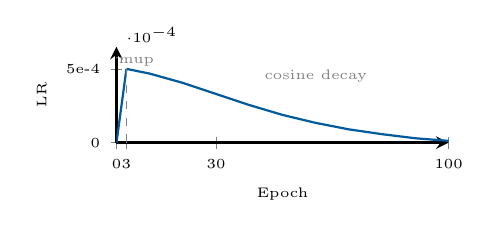
\begin{tikzpicture}
        \begin{axis}[
            width=5.8cm, height=2.8cm,
            xlabel={\tiny Epoch}, ylabel={\tiny LR},
            xtick={0,3,30,100}, xticklabels={\tiny 0,\tiny 3,\tiny 30,\tiny 100},
            ytick={0,0.0005}, yticklabels={\tiny 0,\tiny 5e-4},
            ymin=0, ymax=0.00065,
            xmin=0, xmax=100,
            tick label style={font=\tiny},
            axis lines=left,
            line width=1pt,
          ]
          % Warmup (0->3)
          \addplot[color=accent, thick] coordinates {(0,0)(3,0.0005)};
          % Cosine decay (3->100) — sampled points
          \addplot[color=accent, thick] coordinates {
            (3,0.0005)(10,0.000468)(20,0.000405)(30,0.000330)
            (40,0.000255)(50,0.000188)(60,0.000134)(70,0.0000900)
            (80,0.0000574)(90,0.0000298)(100,0.0000123)
          };
          \draw[dashed, gray, thin] (axis cs:3,0) -- (axis cs:3,0.0005);
          \node[font=\tiny, gray] at (axis cs:1.5,0.00055) {warmup};
          \node[font=\tiny, gray] at (axis cs:60,0.00045) {cosine decay};
        \end{axis}
      \end{tikzpicture}
    \end{column}
    \begin{column}{0.46\textwidth}
      \vspace{2pt}
      {\small\textbf{Early stopping evolution:}}
      \vspace{3pt}

      \begin{center}
      {\small
      \begin{tabular}{lll}
        \toprule
        Run & Stop criterion & Outcome \\
        \midrule
        652 & \texttt{val\_loss} & Stopped epoch 12 \\
            &                   & AP still rising \\
        \midrule
        653+ & \textbf{AP@50}   & Correct behaviour \\
             & patience=10      & Best AP saved \\
        \bottomrule
      \end{tabular}
      }
      \end{center}

      \vspace{8pt}
      {\small\textbf{Hyperparameter changes:}}
      \vspace{3pt}

      \begin{center}
      {\small
      \begin{tabular}{lll}
        \toprule
        Param & Before & After \\
        \midrule
        LR & 1e-3 & 5e-4 \\
        Weight decay & 5e-4 & 1e-3 \\
        min\_delta & 0.05 & 0.001 \\
        \bottomrule
      \end{tabular}
      }
      \end{center}
    \end{column}
  \end{columns}
\end{frame}

% ── SLIDE 5 — Augmentation ───────────────────────────────────────────────────
\begin{frame}{Ultrasound-Specific Data Augmentation}
  \begin{columns}[T]
    \begin{column}{0.48\textwidth}
      \begin{center}
      {\small
      \begin{tabular}{lll}
        \toprule
        Augmentation & Type & Simulates \\
        \midrule
        H/V Flip              & Spatial   & Probe orientation \\
        ShiftScaleRotate      & Spatial   & Probe angle \\
        \rowcolor{rowhl}
        RandomBrightness      & Intensity & Gain / TGC \\
        \rowcolor{rowhl}
        MedianBlur            & Intensity & Speckle suppression \\
        \rowcolor{rowhl}
        MultiplicativeNoise   & Intensity & Speckle (multiplicative) \\
        \rowcolor{rowhl}
        CLAHE                 & Intensity & Contrast norm. \\
        \rowcolor{rowhl}
        RandomGamma           & Intensity & Probe sensitivity \\
        \bottomrule
      \end{tabular}
      }
      \end{center}
      \vspace{4pt}
      {\footnotesize \colorbox{rowhl}{\phantom{x}} US-specific; GaussianBlur/GaussNoise replaced by speckle-physics alternatives}
    \end{column}
    \begin{column}{0.48\textwidth}
      % TikZ: augmentation pipeline
      {\small\textbf{Augmentation pipeline:}}
      \vspace{4pt}

      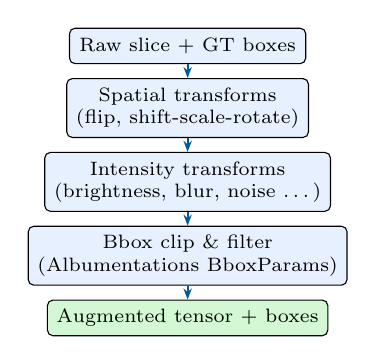
\begin{tikzpicture}[
          node distance=3pt,
          box/.style={draw, rounded corners=2pt, minimum width=3.0cm, minimum height=0.45cm,
                      font=\scriptsize, align=center, fill=blockbg},
          arr/.style={-{Stealth[length=4pt]}, thick, color=accent},
        ]
        \node[box] (raw)  {Raw slice + GT boxes};
        \node[box, below=5pt of raw] (sp)   {Spatial transforms\\(flip, shift-scale-rotate)};
        \node[box, below=5pt of sp]  (int)  {Intensity transforms\\(brightness, blur, noise \ldots)};
        \node[box, below=5pt of int] (bbox) {Bbox clip \& filter\\(Albumentations BboxParams)};
        \node[box, below=5pt of bbox, fill=headgreen!40] (out) {Augmented tensor + boxes};

        \draw[arr] (raw)  -- (sp);
        \draw[arr] (sp)   -- (int);
        \draw[arr] (int)  -- (bbox);
        \draw[arr] (bbox) -- (out);
      \end{tikzpicture}

      \vspace{5pt}
      \begin{block}{\small Speckle physics}
        \scriptsize \textbf{MedianBlur} (not GaussianBlur): edge-preserving non-linear filter — matches clinical speckle reduction; preserves lesion boundaries. \textbf{MultiplicativeNoise} (not GaussNoise): US speckle is \emph{multiplicative} — $I \leftarrow I \times U[0.9,\,1.1]$, not additive.
      \end{block}
      \vspace{4pt}
      \begin{alertblock}{\small No Dropout}
        \scriptsize BN + Dropout interact destructively. Regularisation via weight decay + augmentation + label smoothing only.
      \end{alertblock}
    \end{column}
  \end{columns}
\end{frame}

% ── SLIDE 6 — Scan-Aware Sampling ────────────────────────────────────────────
\begin{frame}{Scan-Aware Slice Sampling}
  \begin{columns}[T]
    \begin{column}{0.50\textwidth}
      \textbf{Problem:} Adjacent ultrasound slices are near-duplicates $\Rightarrow$ redundant gradient updates.

      \vspace{6pt}
      % TikZ: scan window diagram
      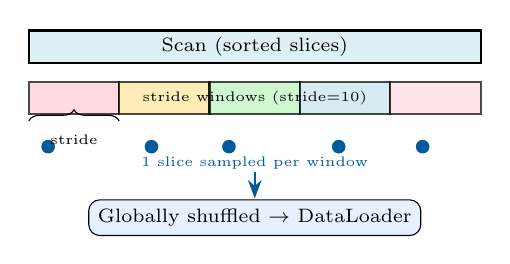
\begin{tikzpicture}[scale=0.82]
        % Scan bar
        \draw[thick, fill=cspblue!40] (0,0) rectangle (7.0,0.5);
        \node[font=\scriptsize] at (3.5,0.25) {Scan (sorted slices)};

        % Windows
        \foreach \x/\col in {0/lossred!70, 1.4/neckyellow!80, 2.8/headgreen!60, 4.2/cspblue!70, 5.6/lossred!50}{
          \draw[thick, fill=\col, opacity=0.7] (\x,-0.8) rectangle (\x+1.4,-0.3);
        }
        \node[font=\tiny] at (3.5,-0.55) {stride windows (stride=10)};

        % Selected slices
        \foreach \x in {0.3, 1.9, 3.1, 4.8, 6.1}{
          \fill[accent] (\x,-1.3) circle (3pt);
        }
        \node[font=\tiny, accent] at (3.5,-1.55) {1 slice sampled per window};

        % Arrow
        \draw[-{Stealth}, thick, accent] (3.5,-1.7) -- (3.5,-2.1);
        \node[draw, rounded corners, fill=blockbg, font=\scriptsize] at (3.5,-2.4) {Globally shuffled $\to$ DataLoader};

        % Brace for stride
        \draw[decorate, decoration={brace,amplitude=4pt}] (0,-0.9) -- (1.4,-0.9);
        \node[font=\tiny, below] at (0.7,-0.96) {stride};
      \end{tikzpicture}
    \end{column}
    \begin{column}{0.46\textwidth}
      \vspace{2pt}
      {\small\textbf{Dataset stats:} 2306 slices, 13 scans, 50 consecutive-slice runs}
      \vspace{4pt}

      \begin{center}
      {\small
      \begin{tabular}{cccc}
        \toprule
        Stride & Slices/epoch & \% total & Per run \\
        \midrule
        5  & $\sim$461 & 20\% & $\sim$6 \\
        \rowcolor{rowhl}
        \textbf{10} & $\sim$\textbf{230} & \textbf{10\%} & $\sim$\textbf{3} \\
        15 & $\sim$154 & 7\%  & $\sim$2 \\
        \bottomrule
      \end{tabular}
      }
      \end{center}
      \vspace{4pt}

      % pgfplot: slices per epoch bar
      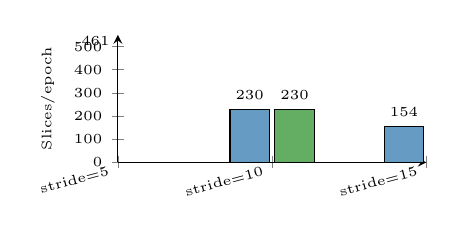
\begin{tikzpicture}
        \begin{axis}[
            ybar, width=5.5cm, height=3.2cm,
            bar width=0.5cm,
            ylabel={\tiny Slices/epoch},
            symbolic x coords={stride=5, stride=10, stride=15},
            xtick=data,
            xticklabel style={font=\tiny, rotate=15, anchor=east},
            yticklabel style={font=\tiny},
            ytick={0,100,200,300,400,500},
            ymin=0, ymax=550,
            nodes near coords,
            nodes near coords style={font=\tiny},
            axis lines=left,
          ]
          \addplot[fill=accent!60] coordinates {
            (stride=5,  461)
            (stride=10, 230)
            (stride=15, 154)
          };
          % Highlight stride=10
          \addplot[fill=good!70] coordinates {(stride=10, 230)};
        \end{axis}
      \end{tikzpicture}
    \end{column}
  \end{columns}
\end{frame}

% Speaker note — Scan-Aware Slice Sampling
\note{
\textbf{Inter-slice redundancy and its effect on training}

\medskip
Ultrasound volumes are acquired by sweeping a transducer continuously across tissue.
At typical clinical acquisition rates the physical distance between adjacent slices is
on the order of 0.5--1\,mm.
At this spacing, the probe has moved so little between frames that the tissue cross-section
is almost identical: the same anatomical structures appear at the same pixel coordinates,
with differences limited to minor speckle fluctuation from micro-vibration and small changes
in acoustic shadowing.

\medskip
\textbf{Why this matters for SGD:}
Each mini-batch gradient update is supposed to represent an independent draw from the data
distribution.
When consecutive slices of the same scan occupy the same batch — or even adjacent batches —
the model effectively sees the same image twice in rapid succession.
The gradient from the second copy nearly cancels any corrective signal from the first,
because the loss has already shifted the weights in exactly the direction that second image
would request.
Concretely, with 2306 slices spread across 50 consecutive-slice runs, naive sequential
sampling means roughly 46 nearly-identical frames follow each other before a scan boundary
is crossed — up to a $\sim$10$\times$ effective reduction in gradient diversity per epoch.

\medskip
\textbf{Downstream effects observed:}
\begin{itemize}
  \item Over-fitting to scan-level texture (speckle patterns, gain settings) rather than lesion morphology.
  \item Artificially low training loss that does not transfer to held-out scans — the validation curve diverges from training loss earlier than expected.
  \item The model learns to suppress predictions in regions that are consistently unannotated \emph{across an entire run}, reinforcing false-negative bias beyond what the labelling rate alone would predict.
\end{itemize}

\medskip
\textbf{The fix — ScanAwareSampler:}
Slices are partitioned into non-overlapping windows of width \texttt{stride} within each scan.
One slice is drawn at random from each window per epoch; the selected slices are then globally
shuffled before entering the DataLoader.
This guarantees a minimum physical separation of \texttt{stride} $\times$ slice-thickness
between any two frames from the same scan that could appear in the same batch,
while still exposing the model to every region of every scan over a sufficient number of epochs.
Stride\,=\,10 reduces per-epoch slice count from 2306 to $\sim$230 — a 10$\times$ diversity gain
at the cost of needing more epochs to achieve full coverage.
}

% ── SLIDE 7 — Mosaic ─────────────────────────────────────────────────────────
\begin{frame}{Cross-Scan Mosaic Augmentation}
  \begin{columns}[T]
    \begin{column}{0.50\textwidth}
      \textbf{Motivation:} $\sim$230 slices/epoch $\Rightarrow$ limited scale \& spatial diversity.\\[4pt]
      Mosaic composites 4 images ($2\times2$ grid) $\Rightarrow$ detection at \textbf{half scale} across varied contexts in one forward pass.

      \vspace{6pt}
      % TikZ: mosaic grid
      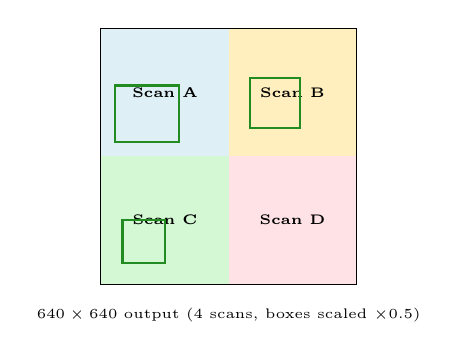
\begin{tikzpicture}[scale=0.9]
        % 2x2 grid
        \draw[thick] (0,0) rectangle (3.6,3.6);
        \draw[thick] (1.8,0) -- (1.8,3.6);
        \draw[thick] (0,1.8) -- (3.6,1.8);

        % Quadrant fills
        \fill[cspblue!40]   (0,1.8)   rectangle (1.8,3.6);
        \fill[neckyellow!50](1.8,1.8) rectangle (3.6,3.6);
        \fill[headgreen!40] (0,0)     rectangle (1.8,1.8);
        \fill[lossred!40]   (1.8,0)   rectangle (3.6,1.8);

        % Scan labels
        \node[font=\tiny\bfseries] at (0.9,2.7) {Scan A};
        \node[font=\tiny\bfseries] at (2.7,2.7) {Scan B};
        \node[font=\tiny\bfseries] at (0.9,0.9) {Scan C};
        \node[font=\tiny\bfseries] at (2.7,0.9) {Scan D};

        % Sample boxes
        \draw[thick, good] (0.2,2.0) rectangle (1.1,2.8);
        \draw[thick, good] (2.1,2.2) rectangle (2.8,2.9);
        \draw[thick, good] (0.3,0.3) rectangle (0.9,0.9);

        % Output label
        \node[font=\tiny, below] at (1.8,-0.2) {$640\times640$ output (4 scans, boxes scaled $\times$0.5)};
      \end{tikzpicture}
    \end{column}
    \begin{column}{0.46\textwidth}
      \vspace{2pt}
      \begin{block}{\small Cross-scan constraint}
        \small 3 mosaic partners always drawn from 3 \emph{different} scan IDs — prevents near-duplicate slices appearing in the same mosaic (would reintroduce redundancy eliminated by ScanAwareSampler).
      \end{block}

      \vspace{4pt}
      {\small\textbf{Implementation path:}}
      \vspace{3pt}

      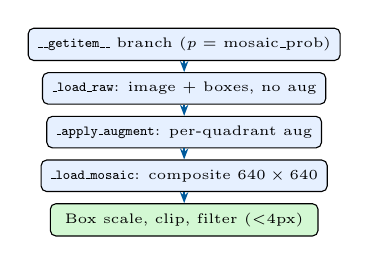
\begin{tikzpicture}[
          node distance=3pt,
          box/.style={draw, rounded corners=2pt, minimum width=3.4cm, minimum height=0.4cm,
                      font=\tiny, align=center, fill=blockbg},
          arr/.style={-{Stealth[length=4pt]}, thick, color=accent},
        ]
        \node[box] (br)  {\texttt{\_\_getitem\_\_} branch ($p=$ mosaic\_prob)};
        \node[box, below=4pt of br] (lr) {\texttt{\_load\_raw}: image + boxes, no aug};
        \node[box, below=4pt of lr] (aa) {\texttt{\_apply\_augment}: per-quadrant aug};
        \node[box, below=4pt of aa] (lm) {\texttt{\_load\_mosaic}: composite $640\times640$};
        \node[box, below=4pt of lm, fill=headgreen!40] (out) {Box scale, clip, filter ($<$4px)};

        \draw[arr] (br)  -- (lr);
        \draw[arr] (lr)  -- (aa);
        \draw[arr] (aa)  -- (lm);
        \draw[arr] (lm)  -- (out);
      \end{tikzpicture}

      \vspace{4pt}
      \textbf{Default:} \texttt{mosaic\_prob=0.5} \quad Val: always 0.0
    \end{column}
  \end{columns}
\end{frame}

% ── SLIDE 8 — Tissue-Aware Copy-Paste ───────────────────────────────────────
\begin{frame}{Tissue-Aware Copy-Paste Augmentation}
  \begin{columns}[T]
    \begin{column}{0.50\textwidth}
      \textbf{Motivation:} Labeled lesion instances are sparse. Copy-paste multiplies GT instances by transplanting existing lesion crops to new tissue-compatible locations — no additional annotation required.

      \vspace{5pt}
      % TikZ: copy-paste pipeline
      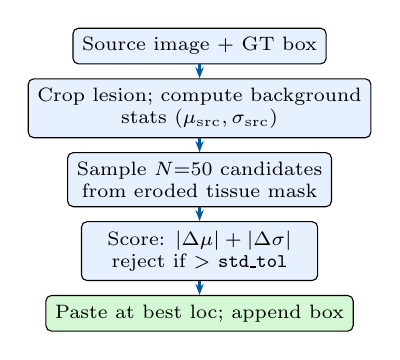
\begin{tikzpicture}[
          node distance=3pt,
          box/.style={draw, rounded corners=2pt, minimum width=3.0cm, minimum height=0.45cm,
                      font=\scriptsize, align=center, fill=blockbg},
          arr/.style={-{Stealth[length=4pt]}, thick, color=accent},
        ]
        \node[box] (src)  {Source image + GT box};
        \node[box, below=5pt of src] (cr)  {Crop lesion; compute background\\stats $(\mu_{\text{src}}, \sigma_{\text{src}})$};
        \node[box, below=5pt of cr]  (sc)  {Sample $N{=}50$ candidates\\from eroded tissue mask};
        \node[box, below=5pt of sc]  (rk)  {Score: $|\Delta\mu|+|\Delta\sigma|$\\reject if $>$ \texttt{std\_tol}};
        \node[box, below=5pt of rk, fill=headgreen!40] (out) {Paste at best loc; append box};
        \draw[arr] (src) -- (cr);
        \draw[arr] (cr)  -- (sc);
        \draw[arr] (sc)  -- (rk);
        \draw[arr] (rk)  -- (out);
      \end{tikzpicture}
    \end{column}
    \begin{column}{0.46\textwidth}
      \vspace{2pt}
      \begin{block}{\small Design choices}
        \small
        \begin{tabular}{ll}
          \toprule
          Choice & Rationale \\
          \midrule
          Tissue mask & Exclude US machine border \\
          Bbox exclusion & Never paste on existing GT \\
          Excl.\ zone $\pm 2r$ & Prevent self-match in scoring \\
          \texttt{std\_tol=25} & Reject tissue-dissimilar locs \\
          \texttt{max\_pastes=2} & Cap augmentation per image \\
          \bottomrule
        \end{tabular}
      \end{block}

      \vspace{4pt}
      \begin{alertblock}{\small Realism vs label validity}
        \scriptsize Pastes need not be physically realistic — only label validity (correct bbox coordinates) is required. The tissue-similarity constraint reduces context mismatch between source and paste.
      \end{alertblock}

      \vspace{4pt}
      {\small\textbf{Config:} \texttt{p=0.4}, \texttt{max\_pastes=2}, \texttt{n\_candidates=50}\\
      Enabled via \texttt{copy\_paste.enabled: true} in YAML.}
    \end{column}
  \end{columns}
\end{frame}

% ── SLIDE 9 — Metrics ────────────────────────────────────────────────────────
\begin{frame}{Evaluation Metrics}
  \begin{columns}[T]
    \begin{column}{0.50\textwidth}
      {\small\textbf{Object-level (primary):} COCO mAP via \texttt{torchmetrics}}

      \vspace{4pt}
      % TikZ PR-curve sketch
      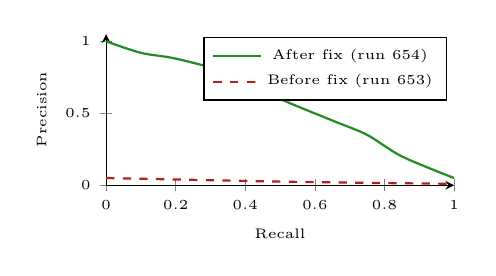
\begin{tikzpicture}
        \begin{axis}[
            width=6cm, height=3.5cm,
            xlabel={\tiny Recall}, ylabel={\tiny Precision},
            xmin=0, xmax=1, ymin=0, ymax=1.05,
            tick label style={font=\tiny},
            axis lines=left,
            legend style={font=\tiny, at={(0.98,0.98)}, anchor=north east},
          ]
          % Stylised PR curve - run 654+ (good)
          \addplot[color=good, thick, smooth] coordinates {
            (0,1)(0.1,0.92)(0.2,0.88)(0.35,0.78)(0.5,0.60)
            (0.65,0.45)(0.75,0.35)(0.85,0.20)(1.0,0.05)
          };
          % Stylised PR curve - run 653 (low precision)
          \addplot[color=bad, thick, dashed, smooth] coordinates {
            (0,0.05)(0.2,0.04)(0.5,0.025)(0.8,0.015)(1.0,0.010)
          };
          \legend{After fix (run 654), Before fix (run 653)}
        \end{axis}
      \end{tikzpicture}
    \end{column}
    \begin{column}{0.46\textwidth}
      \vspace{2pt}
      {\small\textbf{Per-slice AP (screening):}}
      \vspace{4pt}

      % Per-slice AP illustration: coloured boxes = GT label, bars = confidence
      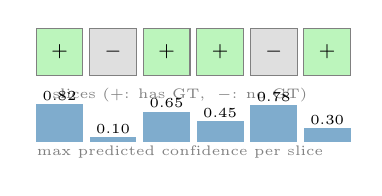
\begin{tikzpicture}[scale=0.85, every node/.style={font=\scriptsize}]
        % GT-positive slices (green)
        \foreach \x in {0, 1.6, 2.4, 4.0}{
          \draw[fill=headgreen!60, draw=gray] (\x,0.5) rectangle (\x+0.7,1.2);
          \node at (\x+0.35,0.85) {$+$};
        }
        % GT-negative slices (gray)
        \foreach \x in {0.8, 3.2}{
          \draw[fill=gray!25, draw=gray] (\x,0.5) rectangle (\x+0.7,1.2);
          \node at (\x+0.35,0.85) {$-$};
        }
        \node[font=\tiny, gray] at (2.15,0.2) {slices ($+$: has GT,\; $-$: no GT)};

        % Confidence bars (height proportional to score)
        \foreach \x/\h/\lbl in {0/0.574/0.82, 0.8/0.070/0.10, 1.6/0.455/0.65,
                                  2.4/0.315/0.45, 3.2/0.546/0.78, 4.0/0.210/0.30}{
          \fill[accent, opacity=0.5] (\x,-0.5) rectangle (\x+0.7, {-0.5+\h});
          \node[font=\tiny] at (\x+0.35, {-0.5+\h+0.12}) {\lbl};
        }
        \node[font=\tiny, gray] at (2.15,-0.65) {max predicted confidence per slice};
      \end{tikzpicture}

      \vspace{4pt}
      \begin{block}{\small Why per-slice AP?}
        \scriptsize Asks \emph{``did the model flag the right frames?''} — robust to partial GT annotations; aligned with radiologist triage workflow.
      \end{block}
    \end{column}
  \end{columns}
\end{frame}

% ── SLIDE 9 — Reproducibility ────────────────────────────────────────────────
\begin{frame}{Full Training Reproducibility}
  \begin{columns}[T]
    \begin{column}{0.50\textwidth}
      Three RNG sources identified and fixed:

      \vspace{6pt}
      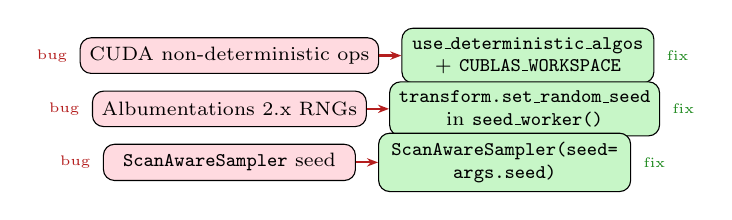
\begin{tikzpicture}[
          node distance=5pt,
          src/.style={draw, fill=lossred!50, rounded corners, minimum width=3.2cm,
                      minimum height=0.45cm, font=\scriptsize, align=center},
          fix/.style={draw, fill=headgreen!50, rounded corners, minimum width=3.2cm,
                      minimum height=0.45cm, font=\scriptsize, align=center},
          arr/.style={-{Stealth[length=4pt]}, thick},
        ]
        \node[src] (c1) {CUDA non-deterministic ops};
        \node[fix, right=8pt of c1] (f1) {\texttt{use\_deterministic\_algos}\\+ \texttt{CUBLAS\_WORKSPACE}};

        \node[src, below=6pt of c1] (c2) {Albumentations 2.x RNGs};
        \node[fix, right=8pt of c2] (f2) {\texttt{transform.set\_random\_seed}\\in \texttt{seed\_worker()}};

        \node[src, below=6pt of c2] (c3) {\texttt{ScanAwareSampler} seed};
        \node[fix, right=8pt of c3] (f3) {\texttt{ScanAwareSampler(seed=}\\\texttt{args.seed)}};

        \draw[arr, bad]  (c1) -- (f1);
        \draw[arr, bad]  (c2) -- (f2);
        \draw[arr, bad]  (c3) -- (f3);

        \node[font=\tiny, bad, left=1pt of c1] {bug};
        \node[font=\tiny, bad, left=1pt of c2] {bug};
        \node[font=\tiny, bad, left=1pt of c3] {bug};
        \node[font=\tiny, good, right=1pt of f1] {fix};
        \node[font=\tiny, good, right=1pt of f2] {fix};
        \node[font=\tiny, good, right=1pt of f3] {fix};
      \end{tikzpicture}
    \end{column}
    \begin{column}{0.46\textwidth}
      \vspace{2pt}
      \begin{block}{\small Seeding hierarchy}
        \begin{center}
        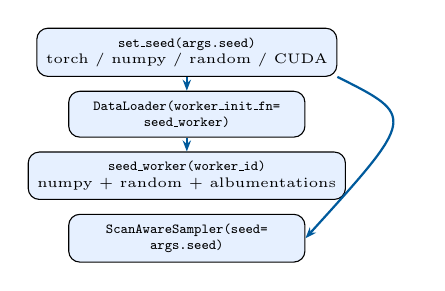
\begin{tikzpicture}[
            node distance=4pt,
            box/.style={draw, rounded corners, fill=blockbg, minimum width=3cm,
                        minimum height=0.4cm, font=\tiny, align=center},
            arr/.style={-{Stealth[length=4pt]}, thick, color=accent},
          ]
          \node[box] (a) {\texttt{set\_seed(args.seed)}\\torch / numpy / random / CUDA};
          \node[box, below=5pt of a] (b) {\texttt{DataLoader(worker\_init\_fn=}\\\texttt{seed\_worker)}};
          \node[box, below=5pt of b] (c) {\texttt{seed\_worker(worker\_id)}\\numpy + random + albumentations};
          \node[box, below=5pt of c] (d) {\texttt{ScanAwareSampler(seed=}\\\texttt{args.seed)}};
          \draw[arr] (a) -- (b);
          \draw[arr] (b) -- (c);
          \draw[arr] (a.south east) .. controls +(1,-0.5) .. (d.east);
        \end{tikzpicture}
        \end{center}
      \end{block}
      \vspace{4pt}
      {\small\textbf{Result:} Same \texttt{--seed} $\Rightarrow$ identical loss curves, metrics, and checkpoints across runs.}
    \end{column}
  \end{columns}
\end{frame}

% ── SLIDE 10 — Results ───────────────────────────────────────────────────────
\begin{frame}{Key Results Across Training Runs}
  \begin{columns}[T]
    \begin{column}{0.50\textwidth}
      \begin{center}
      {\small
      \begin{tabular}{clcc}
        \toprule
        Run & Key change & AP@50 & Prec \\
        \midrule
        650 & Baseline               & unstable & --- \\
        652 & BN fix + grad clip     & 0.507 & low \\
        653 & Early stop on AP       & 0.430 & 1--3\% \\
        \rowcolor{rowhl}
        654 & \textbf{Loss norm fix} & \textbf{0.404}$^*$ & \textbf{40--52\%} \\
        655 & Label smoothing        & pending & pending \\
        \bottomrule
      \end{tabular}
      }
      \end{center}
      {\tiny $^*$ reached by epoch 3; previously epoch 10}

      \vspace{6pt}
      % Precision bar chart
      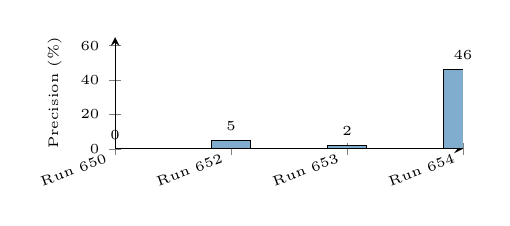
\begin{tikzpicture}
        \begin{axis}[
            ybar, width=6cm, height=3.0cm,
            bar width=0.5cm,
            ylabel={\tiny Precision (\%)},
            symbolic x coords={Run 650, Run 652, Run 653, Run 654},
            xtick=data,
            xticklabel style={font=\tiny, rotate=20, anchor=east},
            yticklabel style={font=\tiny},
            ymin=0, ymax=65,
            nodes near coords,
            nodes near coords style={font=\tiny},
            axis lines=left,
          ]
          \addplot[fill=accent!50] coordinates {
            (Run 650,0)(Run 652,5)(Run 653,2)(Run 654,46)
          };
        \end{axis}
      \end{tikzpicture}
    \end{column}
    \begin{column}{0.46\textwidth}
      \vspace{2pt}
      {\small\textbf{AP@50 convergence speed — loss norm fix:}}
      \vspace{4pt}

      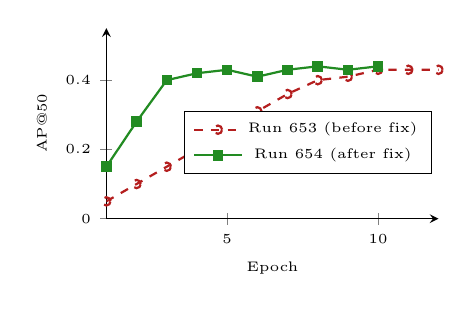
\begin{tikzpicture}
        \begin{axis}[
            width=5.8cm, height=4.0cm,
            xlabel={\tiny Epoch},
            ylabel={\tiny AP@50},
            xmin=1, xmax=12,
            ymin=0, ymax=0.55,
            tick label style={font=\tiny},
            axis lines=left,
            legend style={font=\tiny, at={(0.98,0.4)}, anchor=east},
          ]
          % Run 653 (slow, low prec)
          \addplot[color=bad, thick, dashed, mark=o, mark size=1.5pt] coordinates {
            (1,0.05)(2,0.10)(3,0.15)(4,0.20)(5,0.26)(6,0.31)
            (7,0.36)(8,0.40)(9,0.41)(10,0.43)(11,0.43)(12,0.43)
          };
          % Run 654 (fast, good prec)
          \addplot[color=good, thick, mark=square*, mark size=1.5pt] coordinates {
            (1,0.15)(2,0.28)(3,0.40)(4,0.42)(5,0.43)(6,0.41)
            (7,0.43)(8,0.44)(9,0.43)(10,0.44)
          };
          \legend{Run 653 (before fix), Run 654 (after fix)}
        \end{axis}
      \end{tikzpicture}
    \end{column}
  \end{columns}
\end{frame}

% ── SLIDE 11 — Next Steps ────────────────────────────────────────────────────
\begin{frame}{Next Steps}
  \begin{columns}[T]
    \begin{column}{0.48\textwidth}
      \textbf{Immediate (run 655 eval)}
      \begin{itemize}
        \item Target: AP@50 $>$ 0.50, Prec $>$ 0.40
        \item If val loss diverges after epoch $\sim$10: increase weight decay or reduce epoch budget
      \end{itemize}

      \vspace{8pt}
      \textbf{Hyperparameter optimisation}
      \begin{itemize}
        \item Systematic sweep: LR, weight decay, label smoothing $\epsilon$, \texttt{mosaic\_prob}
        \item \texttt{slice\_stride} ablation vs mAP / convergence speed
      \end{itemize}

      \vspace{8pt}
      \textbf{PU-Loss investigation}
      \begin{itemize}
        \item Diagnose mAP degradation vs baseline
        \item Gradient re-weighting interaction with DFL
      \end{itemize}
    \end{column}
    \begin{column}{0.48\textwidth}
      \textbf{Semi-supervised / pseudo-labeling}

      \vspace{4pt}
      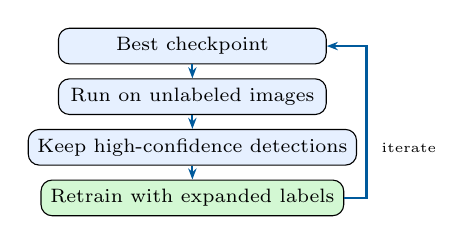
\begin{tikzpicture}[
          node distance=5pt,
          box/.style={draw, rounded corners, fill=blockbg, minimum width=3.4cm,
                      minimum height=0.45cm, font=\scriptsize, align=center},
          arr/.style={-{Stealth[length=4pt]}, thick, color=accent},
        ]
        \node[box] (m) {Best checkpoint};
        \node[box, below=5pt of m] (u) {Run on unlabeled images};
        \node[box, below=5pt of u] (f) {Keep high-confidence detections};
        \node[box, below=5pt of f, fill=headgreen!40] (r) {Retrain with expanded labels};
        \draw[arr] (m) -- (u);
        \draw[arr] (u) -- (f);
        \draw[arr] (f) -- (r);
        \draw[arr] (r.east) -- ++(8pt,0) |- (m.east);
        \node[font=\tiny, right=10pt of r, yshift=18pt] {iterate};
      \end{tikzpicture}

      \vspace{8pt}
      \textbf{Evaluation}
      \begin{itemize}
        \item Report per-slice AP@50 alongside object-level AP
        \item Calibration analysis (confidence vs actual precision)
      \end{itemize}
    \end{column}
  \end{columns}
\end{frame}

% ── SLIDE 12 — Summary ───────────────────────────────────────────────────────
\begin{frame}{Summary}
  \begin{center}
    \large\textbf{From unstable training to reproducible, precision-aware detection}
  \end{center}

  \vspace{4pt}

  % Timeline of milestones
  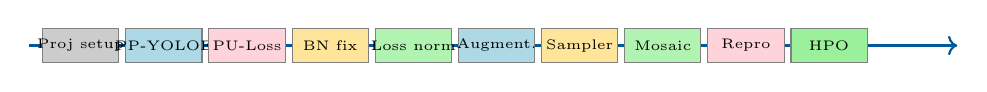
\begin{tikzpicture}[scale=0.88]
    \draw[thick, ->, accent] (0,0) -- (13.4,0);
    \foreach \x/\lbl/\col in {
        0.2/Proj setup/gray!40,
        1.4/PP-YOLOE/cspblue,
        2.6/PU-Loss/lossred!60,
        3.8/BN fix/neckyellow!80,
        5.0/Loss norm/headgreen!70,
        6.2/Augment./cspblue,
        7.4/Sampler/neckyellow!80,
        8.6/Mosaic/headgreen!70,
        9.8/Repro/lossred!60,
        11.0/HPO/headgreen!90
    }{
      \fill[\col, draw=gray] (\x,-0.25) rectangle (\x+1.1,0.25);
      \node[font=\tiny, align=center] at (\x+0.55,0) {\lbl};
    }
  \end{tikzpicture}

  \vspace{6pt}

  \begin{columns}[T]
    \begin{column}{0.48\textwidth}
      \textbf{What we built}
      \begin{itemize}\small
        \item PP-YOLOE adapted for ultrasound OD
        \item PU-Loss for partially-labeled data
        \item Scan-aware sampler ($\sim$10$\times$ redundancy reduction)
        \item Cross-scan mosaic augmentation
        \item Dual metrics: object-level + slice-level AP
        \item Fully deterministic, seed-controlled training
      \end{itemize}
    \end{column}
    \begin{column}{0.48\textwidth}
      \textbf{Key lessons}
      \begin{itemize}\small
        \item \textbf{Loss normalisation} is the single highest-leverage fix\\
              {\color{bad}2\%} $\to$ {\color{good}50\%} precision
        \item BN mode during validation silently corrupts metrics
        \item Grayscale US $\neq$ RGB — domain augmentations matter
        \item Reproducibility needs all 3 RNG sources seeded
      \end{itemize}
    \end{column}
  \end{columns}
\end{frame}

% ══════════════════════════════════════════════════════════════════════════════
%  SECTION: Hyperparameter Optimisation
% ══════════════════════════════════════════════════════════════════════════════

% ── SLIDE HPO-1 — Optuna Setup ───────────────────────────────────────────────
\begin{frame}{Hyperparameter Optimisation — Optuna Setup}
  \begin{columns}[T]
    \begin{column}{0.50\textwidth}
      \textbf{Objective:} Maximise val AP@50 over 50-epoch short runs.\\[4pt]
      \textbf{Framework:} Optuna (TPE sampler, MedianPruner)\\
      \textbf{Scale:} 12 parallel SLURM workers, shared SQLite study on NFS.

      \vspace{6pt}
      \begin{block}{\small Search space}
        \small
        \begin{tabular}{ll}
          \toprule
          Parameter & Range / Choices \\
          \midrule
          \texttt{learning\_rate}   & \texttt{log-uniform}$[10^{-4},5{\times}10^{-3}]$ \\
          \texttt{weight\_decay}    & \texttt{log-uniform}$[10^{-4},10^{-2}]$ \\
          \texttt{slice\_stride}    & $\{5, 7, 10\}$ \\
          \texttt{batch\_size}      & $\{8, 16, 32\}$ \\
          \texttt{mosaic\_prob}     & \texttt{uniform}$[0.1, 0.5]$ \\
          \texttt{label\_smooth}    & \texttt{uniform}$[0.0, 0.15]$ \\
          \texttt{use\_clahe}       & \{True, False\} \\
          \texttt{use\_ssr}         & \{True, False\} \\
          \texttt{use\_rbc}         & \{True, False\} \\
          \bottomrule
        \end{tabular}
      \end{block}
    \end{column}
    \begin{column}{0.46\textwidth}
      \vspace{2pt}
      \begin{block}{\small Study statistics — Job 710}
        \small
        \begin{tabular}{ll}
          \toprule
          Metric & Value \\
          \midrule
          Total trials launched & 120 \\
          \rowcolor{rowhl}
          Completed & 35 \\
          Pruned (MedianPruner) & 85 \\
          Failed & 0 \\
          \midrule
          Epochs per trial (max) & 50 \\
          Early-stop patience & 25 ep \\
          Prune warmup steps & 10 ep \\
          \midrule
          \rowcolor{rowhl}
          \textbf{Best AP@50} & \textbf{0.5787} \\
          Best trial \# & 60 \\
          \bottomrule
        \end{tabular}
      \end{block}

      \vspace{4pt}
      {\small\textbf{Pruning efficiency:} 71\% of trials pruned early, saving $\sim$3$\times$ compute vs running all 120 to 50 epochs.}
    \end{column}
  \end{columns}
\end{frame}

% ── SLIDE HPO-2 — Optimization History ──────────────────────────────────────
\begin{frame}{HPO — Optimization History}
  \begin{columns}[T]
    \begin{column}{0.58\textwidth}
      \begin{center}
        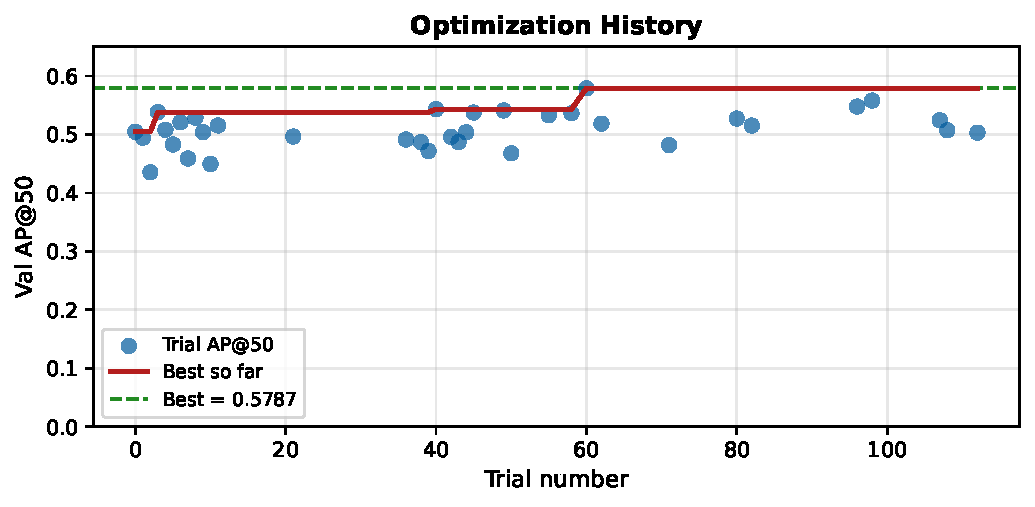
\includegraphics[width=\linewidth]{figures/optim_history.pdf}
      \end{center}
    \end{column}
    \begin{column}{0.39\textwidth}
      \vspace{8pt}
      \textbf{Key observations:}
      \begin{itemize}\small
        \item TPE sampler converges rapidly: best-so-far curve plateaus after $\sim$60 trials
        \item Peak: \textbf{AP@50 = 0.5787} (trial \#60)
        \item Completed trials cluster tightly in $[0.49, 0.58]$ once pruner eliminates bad configs
        \item Trials \#0--8 were warmup for the MedianPruner (8 startup trials required before pruning activates)
      \end{itemize}

      \vspace{4pt}
      \begin{alertblock}{\small Baseline reference}
        \scriptsize Pre-HPO best run (Job 654): AP@50 $\approx$ 0.404 at epoch 3. HPO yields a \textbf{+17.8 pp} gain with a principled config.
      \end{alertblock}
    \end{column}
  \end{columns}
\end{frame}

% ── SLIDE HPO-3 — Best Configuration ─────────────────────────────────────────
\begin{frame}{HPO — Best Hyperparameter Configuration}
  \begin{columns}[T]
    \begin{column}{0.50\textwidth}
      \begin{block}{\small Best trial (\#60) — AP@50 = 0.5787}
        \small
        \begin{tabular}{lll}
          \toprule
          Parameter & Best Value & Prior guess \\
          \midrule
          \texttt{learning\_rate}   & $6.08 \times 10^{-4}$ & $5 \times 10^{-4}$ \\
          \rowcolor{rowhl}
          \texttt{weight\_decay}    & $9.69 \times 10^{-3}$ & $1 \times 10^{-3}$ \\
          \texttt{slice\_stride}    & $5$ & $10$ \\
          \rowcolor{rowhl}
          \texttt{batch\_size}      & $32$ & $32$ \\
          \texttt{mosaic\_prob}     & $0.36$ & $0.50$ \\
          \rowcolor{rowhl}
          \texttt{label\_smooth}    & $0.098$ & $0.10$ \\
          \texttt{use\_clahe}       & \color{bad}False & True \\
          \rowcolor{rowhl}
          \texttt{use\_ssr}         & \color{good}True & True \\
          \texttt{use\_rbc}         & \color{bad}False & True \\
          \bottomrule
        \end{tabular}
      \end{block}
    \end{column}
    \begin{column}{0.46\textwidth}
      \vspace{2pt}
      \textbf{Surprises vs prior config:}
      \begin{itemize}\small
        \item \textbf{Weight decay $10\times$ higher} than prior ($9.7 \times 10^{-3}$ vs $10^{-3}$) — stronger regularisation beneficial on small dataset
        \item \textbf{CLAHE \& RBC both off:} contrast normalisation at inference time; brightness changes at train time adds noise for our scanner type
        \item \textbf{Stride = 5} consistently preferred over 10 — denser sampling outweighs slice redundancy at 50-epoch budget
        \item \textbf{Mosaic prob $\approx$ 0.35} vs 0.50 default — confirms partial mosaic better than always-on
      \end{itemize}

      \vspace{4pt}
      {\small\textbf{Top-5 configs saved} to \texttt{train/config/hparam\_rank*.yaml}; best config deployed as \texttt{best\_hparams.yaml}.}
    \end{column}
  \end{columns}
\end{frame}

% ── SLIDE HPO-4 — LR and WD Analysis ─────────────────────────────────────────
\begin{frame}{HPO — Learning Rate \& Weight Decay}
  \begin{center}
    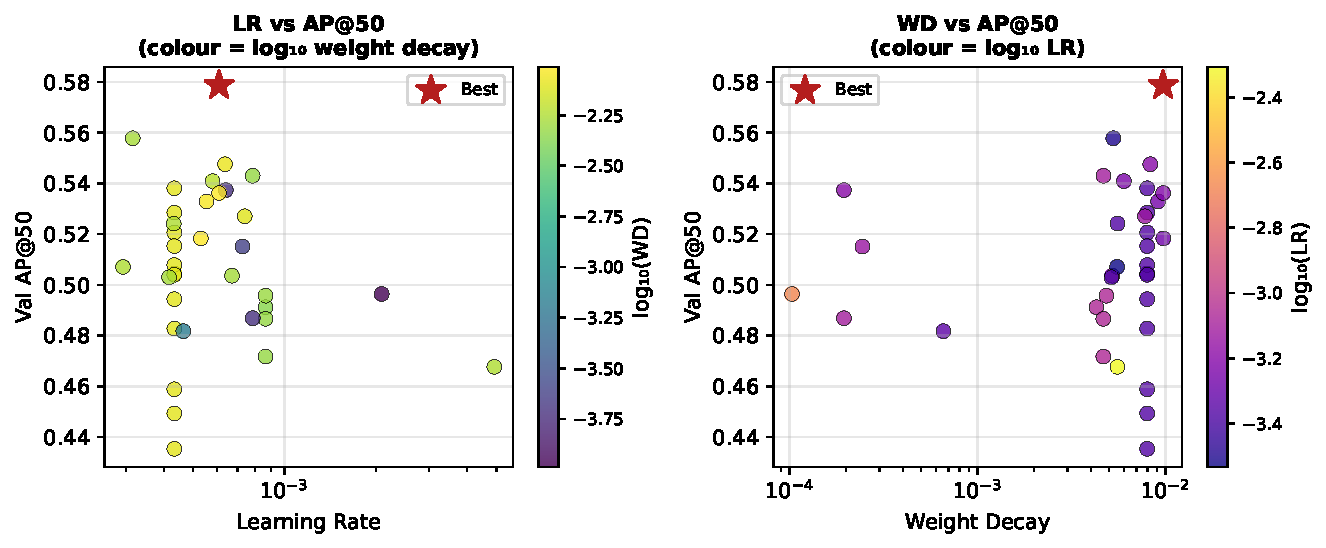
\includegraphics[width=0.92\linewidth]{figures/lr_wd_scatter.pdf}
  \end{center}
  \vspace{-4pt}
  \begin{columns}[T]
    \begin{column}{0.48\textwidth}
      {\small\textbf{LR:} Best performance in $[4 \times 10^{-4},\; 8 \times 10^{-4}]$. Very high LR ($>10^{-3}$) degrades AP@50. The star marks the best trial.}
    \end{column}
    \begin{column}{0.48\textwidth}
      {\small\textbf{WD:} Higher weight decay ($>5 \times 10^{-3}$) correlates with top scores. Spearman $\rho = 0.28$ — moderate positive trend. Acts as additional regularisation for the small US dataset.}
    \end{column}
  \end{columns}
\end{frame}

% ── SLIDE HPO-5 — Categorical Parameters ─────────────────────────────────────
\begin{frame}{HPO — Categorical Parameter Analysis}
  \begin{center}
    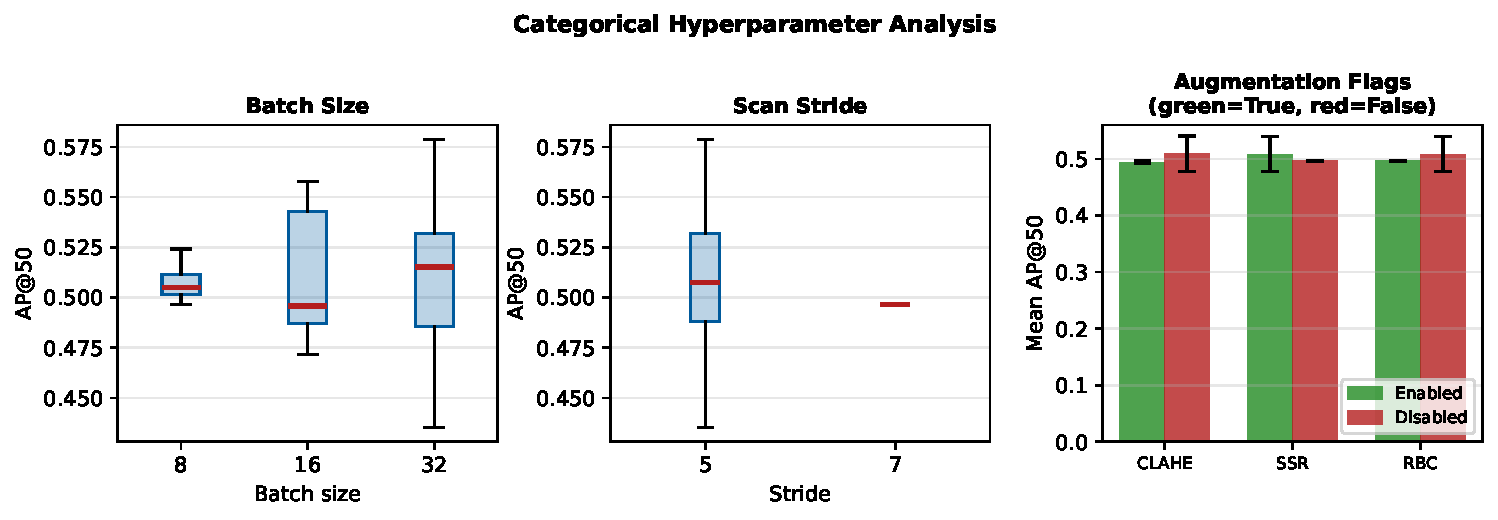
\includegraphics[width=0.90\linewidth]{figures/categorical_analysis.pdf}
  \end{center}
  \vspace{-4pt}
  \begin{columns}[T]
    \begin{column}{0.32\textwidth}
      {\small\textbf{Batch size:} All three options perform similarly. Batch 32 has the widest spread and the highest peak — larger batches give more stable gradient estimates.}
    \end{column}
    \begin{column}{0.32\textwidth}
      {\small\textbf{Slice stride:} Stride = 5 dominates with 34/35 completed trials. The single stride = 7 trial scored 0.496. Stride = 10 consistently pruned early — too sparse for 50-epoch runs.}
    \end{column}
    \begin{column}{0.32\textwidth}
      {\small\textbf{Augmentation flags:} SSR (ShiftScaleRotate) \emph{enabled} is universally beneficial. CLAHE and RBC show minimal benefit and are off in all top-ranked configs.}
    \end{column}
  \end{columns}
\end{frame}

% ── SLIDE HPO-6 — Continuous Parameters ──────────────────────────────────────
\begin{frame}{HPO — Mosaic Probability \& Label Smoothing}
  \begin{center}
    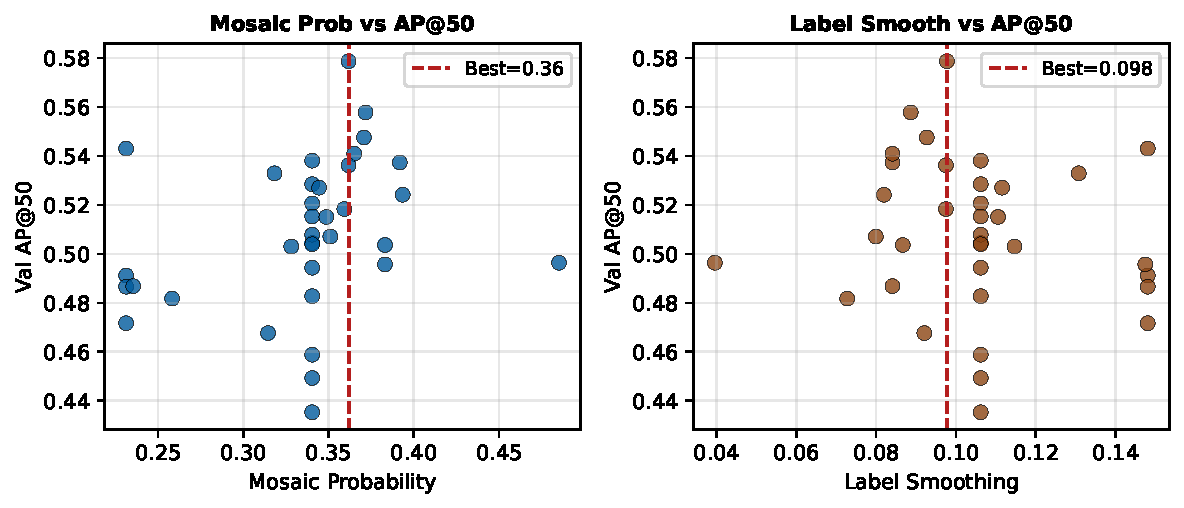
\includegraphics[width=0.80\linewidth]{figures/continuous_params.pdf}
  \end{center}
  \vspace{-4pt}
  \begin{columns}[T]
    \begin{column}{0.50\textwidth}
      {\small\textbf{Mosaic probability} shows the strongest correlation with AP@50 (Spearman $\rho = 0.447$, $p = 0.007$). Optimal range $[0.30, 0.42]$. Very low mosaic prob ($<0.2$) consistently underperforms. The dashed line marks the best trial value (0.36).}
    \end{column}
    \begin{column}{0.46\textwidth}
      {\small\textbf{Label smoothing} shows weak correlation ($\rho = -0.15$, $p = 0.39$). Performance is relatively flat across the search range $[0, 0.15]$. The best trial used $\varepsilon = 0.098$ — mild smoothing reduces overconfident predictions on noisy US labels.}
    \end{column}
  \end{columns}
\end{frame}

% ── SLIDE HPO-7 — Hyperparameter Importance ──────────────────────────────────
\begin{frame}{HPO — Hyperparameter Importance}
  \begin{columns}[T]
    \begin{column}{0.52\textwidth}
      \begin{center}
        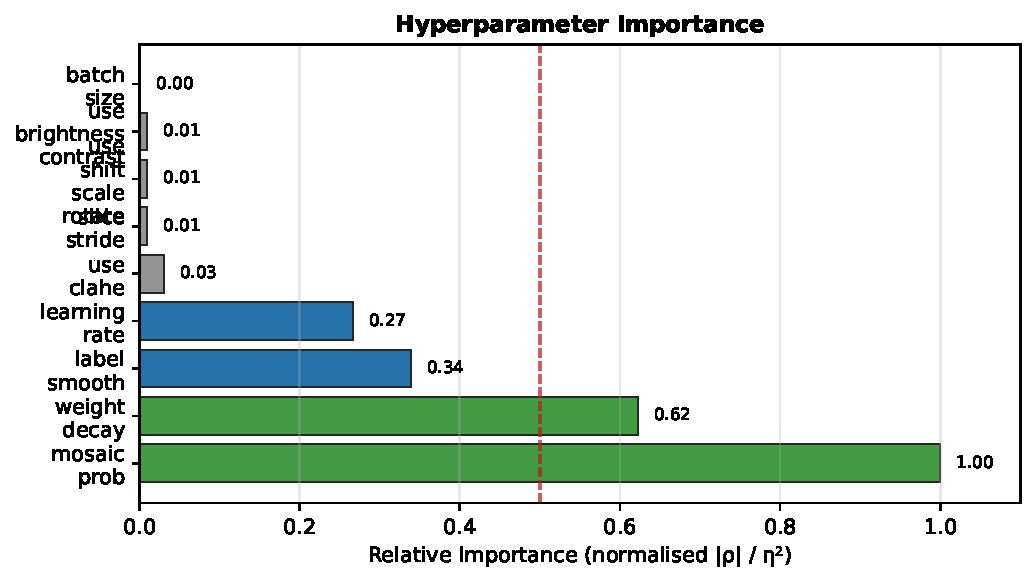
\includegraphics[width=\linewidth]{figures/hparam_importance.pdf}
      \end{center}
    \end{column}
    \begin{column}{0.44\textwidth}
      \vspace{6pt}
      \textbf{Importance metric:}\\
      {\small Continuous params: $|\rho_{\text{Spearman}}|$ between param value and AP@50.\\
      Categorical params: $\eta^2$ (ratio of between-group SS to total SS in AP@50).\\
      Values normalised to $[0, 1]$.}

      \vspace{8pt}
      \textbf{Ranking summary:}
      \begin{enumerate}\small
        \item \textbf{Mosaic prob} — strongest continuous signal ($\rho=0.45$, $p<0.01$)
        \item \textbf{Slice stride} — structural choice; stride 5 dominates
        \item \textbf{Weight decay} — higher WD beneficial ($\rho=0.28$)
        \item \textbf{Batch size} — weak effect once large enough
        \item \textbf{Augmentation flags} — SSR important; CLAHE/RBC negligible
        \item \textbf{LR, label smooth} — insensitive within feasible range
      \end{enumerate}

      \vspace{4pt}
      {\small\textbf{Takeaway:} Data pipeline choices (mosaic, stride) matter more than optimiser micro-tuning for this dataset size.}
    \end{column}
  \end{columns}
\end{frame}

% ── SLIDE HPO-8 — Best Trial Learning Curves ─────────────────────────────────
\begin{frame}{HPO — Best Trial Learning Curves (Trial \#60)}
  \begin{columns}[T]
    \begin{column}{0.55\textwidth}
      \begin{center}
        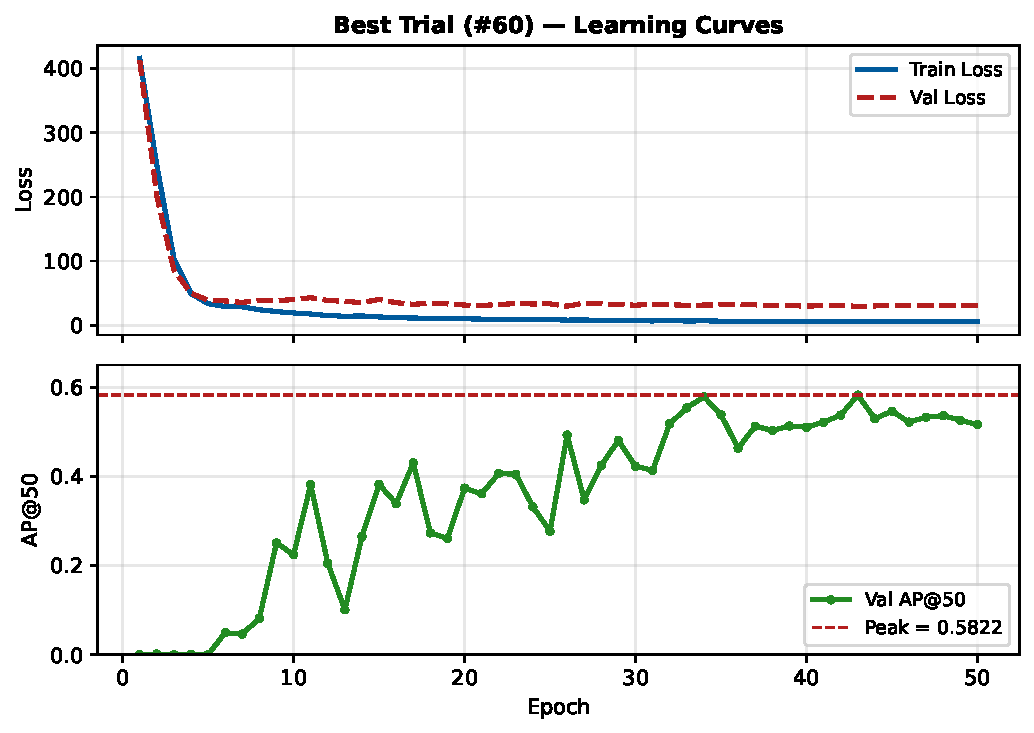
\includegraphics[width=\linewidth]{figures/best_trial_curves.pdf}
      \end{center}
    \end{column}
    \begin{column}{0.41\textwidth}
      \vspace{6pt}
      \textbf{Config:}\\
      {\small lr=$6.1 \times 10^{-4}$, wd=$9.7 \times 10^{-3}$\\
      stride=5, bs=32, mosaic=0.36\\
      ls=0.098, CLAHE=off, SSR=on, RBC=off}

      \vspace{8pt}
      \textbf{Training dynamics:}
      \begin{itemize}\small
        \item Warmup (8 epochs) smoothly ramps LR from $6 \times 10^{-5}$
        \item AP@50 crosses 0.50 at epoch $\sim$20 and steadily improves
        \item Train loss decreases cleanly — no instability or gradient spikes
        \item Val loss plateaus at $\sim$31 from epoch 20 onwards while AP@50 keeps climbing — \textbf{no overfitting}
        \item Peak AP@50 = \textbf{0.5787} at epoch 41
        \item Run completes all 50 epochs (no early stop triggered)
      \end{itemize}

      \vspace{4pt}
      \begin{block}{\small vs. baseline}
        \scriptsize Job 654 (pre-HPO): AP@50 $\approx$ 0.40\\
        Best HPO trial: AP@50 = \textbf{0.579} \quad {\color{good}$\uparrow$45\%}
      \end{block}
    \end{column}
  \end{columns}
\end{frame}

% ══════════════════════════════════════════════════════════════════════════════
%  SECTION: Baseline vs PU Loss — Full Training Comparison
% ══════════════════════════════════════════════════════════════════════════════

% ── SLIDE CMP-1 — Setup ───────────────────────────────────────────────────────
\begin{frame}{Baseline vs PU Loss — Experimental Setup}
  \begin{columns}[T]
    \begin{column}{0.50\textwidth}
      \textbf{Objective:} Compare standard cross-entropy loss against PU-aware focal loss using the best hyperparameters found by Optuna.

      \vspace{6pt}
      \begin{block}{\small Shared configuration (both runs)}
        \small
        \begin{tabular}{ll}
          \toprule
          Parameter & Value \\
          \midrule
          LR & $6.08 \times 10^{-4}$ \\
          Weight decay & $9.69 \times 10^{-3}$ \\
          Slice stride & 5 \\
          Batch size & 32 \\
          Mosaic prob & 0.36 \\
          Label smoothing & 0.098 \\
          Warmup epochs & 8 \\
          Max epochs & 100 \\
          Early-stop patience & 20 ep \\
          \bottomrule
        \end{tabular}
      \end{block}
    \end{column}
    \begin{column}{0.46\textwidth}
      \vspace{2pt}
      \begin{block}{\small Run summary}
        \small
        \begin{tabular}{lll}
          \toprule
          & \textbf{Baseline} & \textbf{PU Loss} \\
          \midrule
          Loss fn      & YOLOELoss & YOLOEPUFocal \\
          Epochs run   & 35        & 77 \\
          Early stop   & ep 35     & ep 77 \\
          \rowcolor{rowhl}
          Best AP@50   & 0.450     & \textbf{0.557} \\
          Best epoch   & 15        & 57 \\
          Train time   & 17 min    & 35 min \\
          \bottomrule
        \end{tabular}
      \end{block}

      \vspace{6pt}
      \begin{alertblock}{\small Key finding}
        \small PU Loss achieves \textbf{+10.7 pp AP@50} over the baseline under identical HPO-tuned configuration, resolving the earlier degradation observed before HPO.
      \end{alertblock}
    \end{column}
  \end{columns}
\end{frame}

% ── SLIDE CMP-2 — Training Curves ─────────────────────────────────────────────
\begin{frame}{Training Curves: Baseline vs PU Loss}
  \begin{center}
    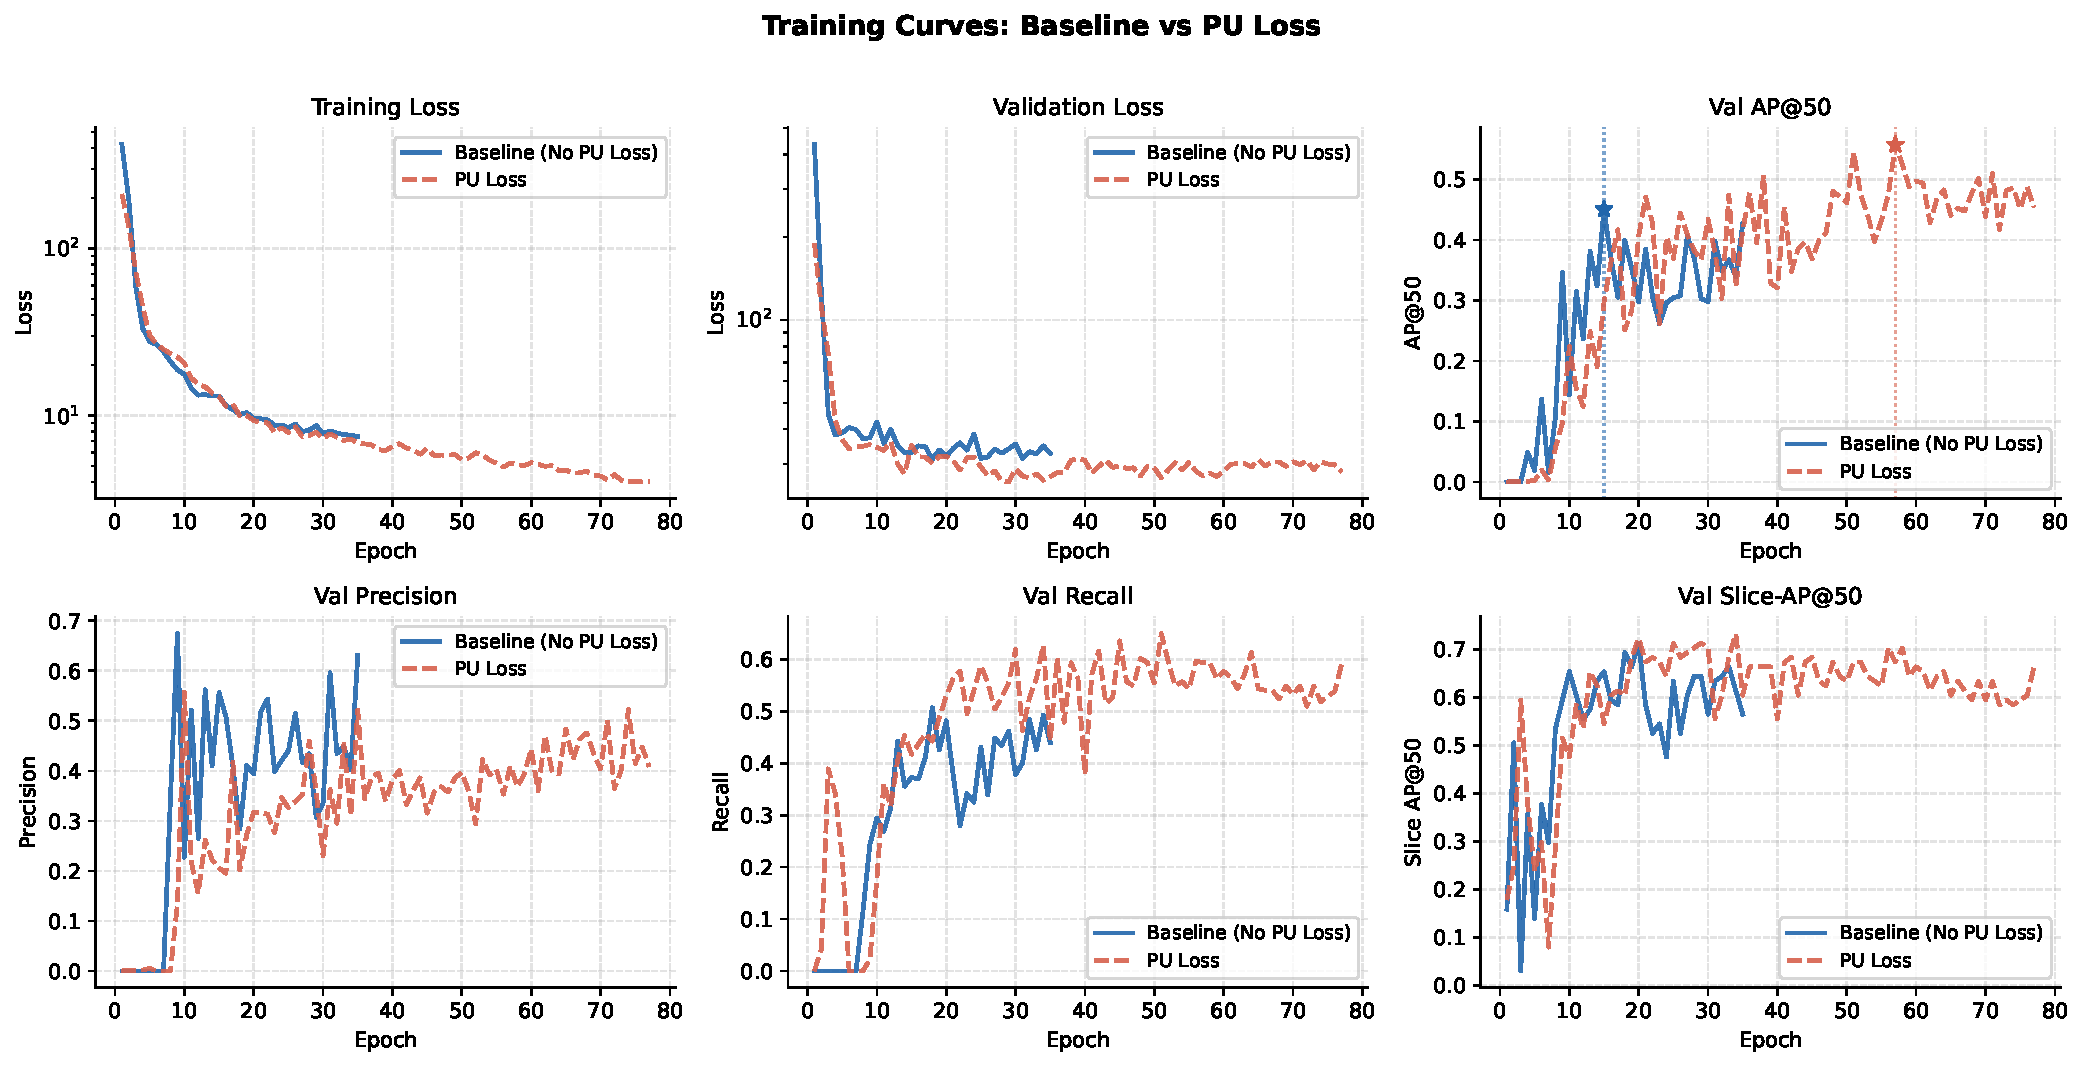
\includegraphics[width=\linewidth]{figures/pu_loss_training_curves.pdf}
  \end{center}
  \vspace{-6pt}
  \begin{columns}[T]
    \begin{column}{0.50\textwidth}
      {\small
      \textbf{Loss (train \& val):} PU Loss shows higher raw loss values due to gradient re-weighting, but val loss stabilises lower after epoch 20.
      Train loss trajectories are qualitatively similar in shape.}
    \end{column}
    \begin{column}{0.46\textwidth}
      {\small
      \textbf{AP@50 \& Slice-AP@50:} PU Loss converges more slowly (best at epoch 57 vs 15) but reaches a substantially higher plateau.
      Stars mark the saved best checkpoint per run.}
    \end{column}
  \end{columns}
\end{frame}

% ── SLIDE CMP-3 — Detection Metrics ───────────────────────────────────────────
\begin{frame}{Detection Metrics: Baseline vs PU Loss}
  \begin{center}
    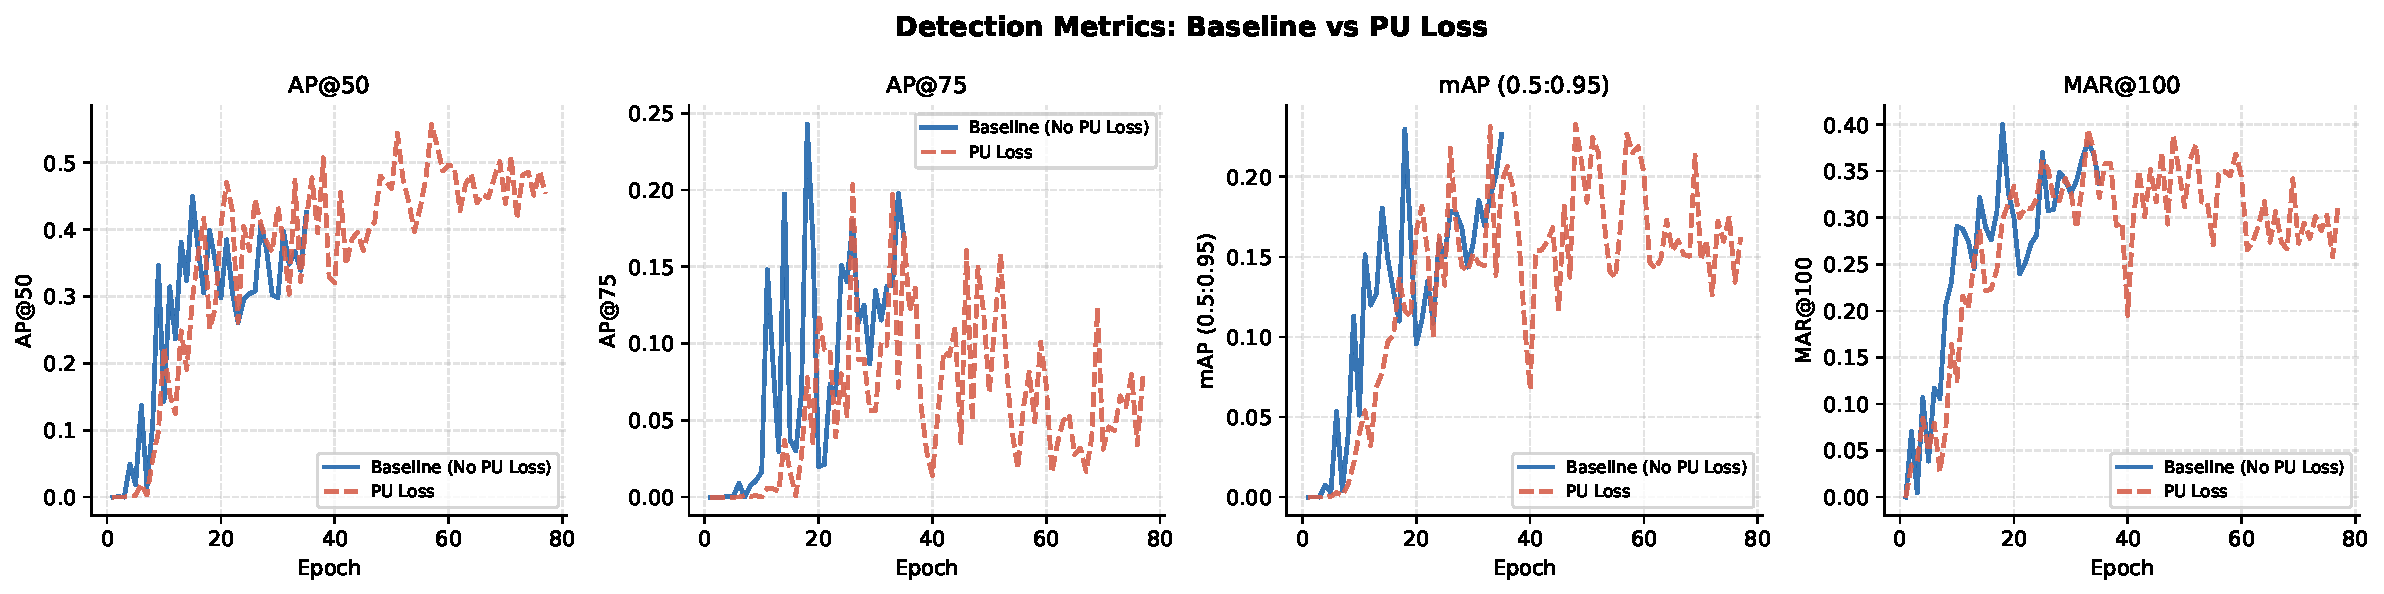
\includegraphics[width=\linewidth]{figures/pu_loss_map_metrics.pdf}
  \end{center}
  \vspace{-6pt}
  \begin{columns}[T]
    \begin{column}{0.50\textwidth}
      {\small
      \textbf{AP@50 \& AP@75:} PU Loss outperforms on both thresholds. AP@75 gap is smaller, suggesting the precision improvement is concentrated at lower IoU thresholds.}
    \end{column}
    \begin{column}{0.46\textwidth}
      {\small
      \textbf{mAP (0.5:0.95) \& MAR@100:} PU Loss achieves higher MAR@100 by epoch 50+, confirming improved recall at higher operating points. mAP gains are more modest but consistent.}
    \end{column}
  \end{columns}
\end{frame}

% ── SLIDE CMP-4 — Summary Bar Chart ───────────────────────────────────────────
\begin{frame}{Peak Metric Comparison: Baseline vs PU Loss}
  \begin{center}
    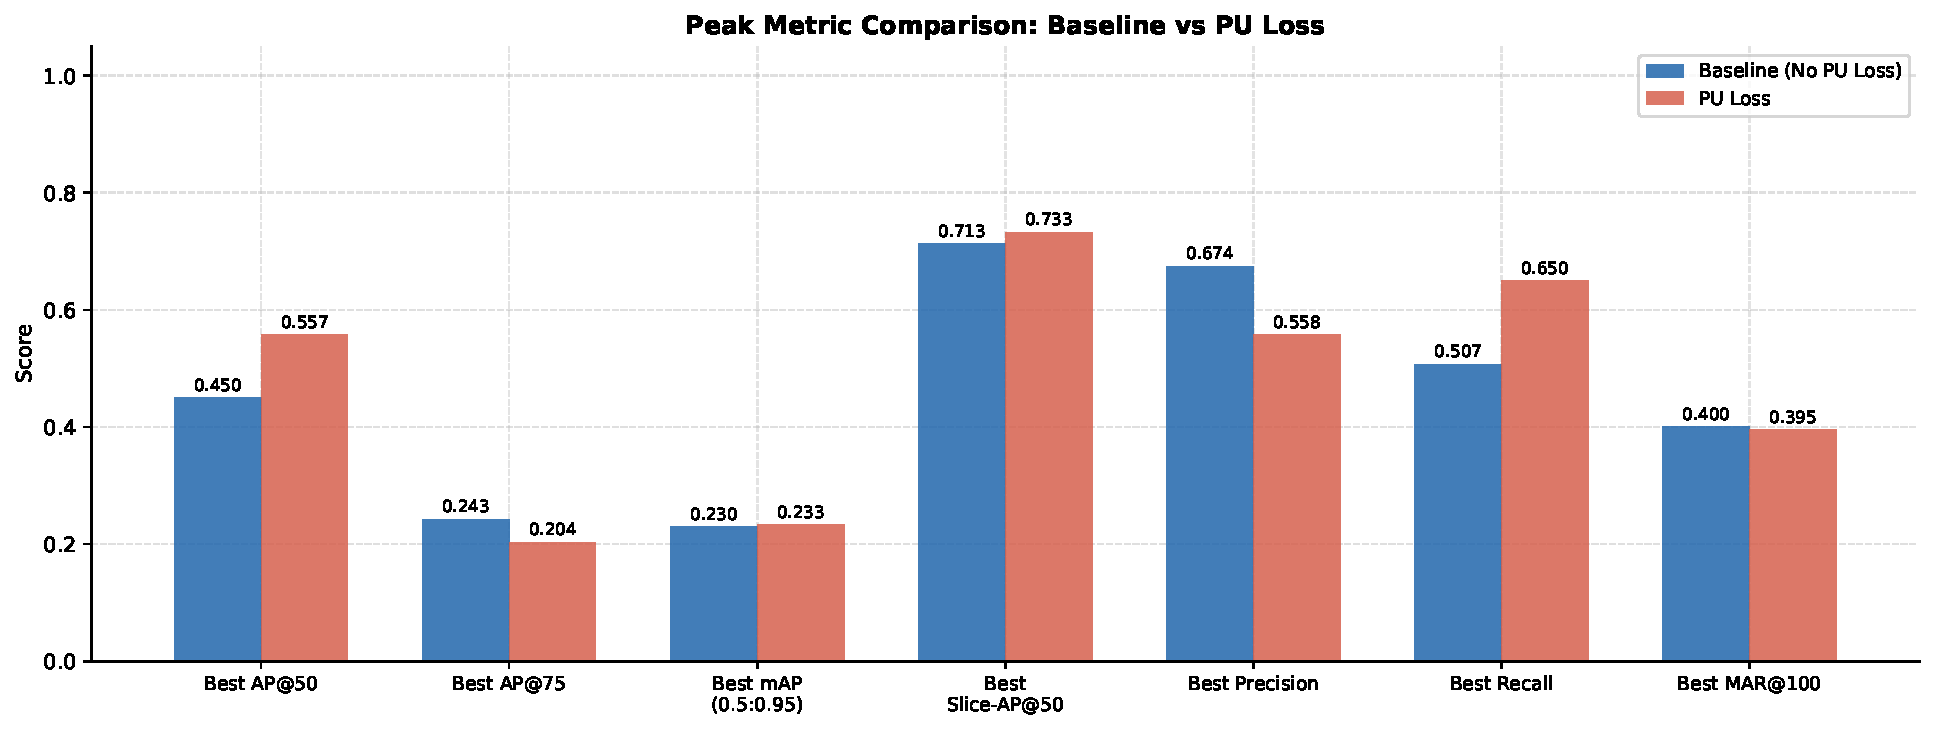
\includegraphics[width=0.95\linewidth]{figures/pu_loss_summary_bar.pdf}
  \end{center}
  \vspace{-6pt}
  {\small
  PU Loss improves AP@50, AP@75, mAP, and recall.
  Precision is comparable across both runs — PU Loss does not sacrifice precision to gain recall.
  Slice-AP@50 advantage of PU Loss (+0.03) is modest but consistent with improved frame-level detection.
  }
\end{frame}

% ── SLIDE CMP-5 — Precision / Recall Analysis ────────────────────────────────
\begin{frame}{Precision–Recall Dynamics: Baseline vs PU Loss}
  \begin{columns}[T]
    \begin{column}{0.50\textwidth}
      {\small\textbf{At best checkpoint:}}
      \vspace{4pt}

      \begin{center}
      {\small
      \begin{tabular}{lccc}
        \toprule
        Run & Precision & Recall & AP@50 \\
        \midrule
        Baseline  & 0.631 & 0.493 & 0.450 \\
        \rowcolor{rowhl}
        PU Loss   & 0.536 & \textbf{0.594} & \textbf{0.557} \\
        \bottomrule
      \end{tabular}
      }
      \end{center}

      \vspace{6pt}
      % pgfplot: precision-recall tradeoff scatter
      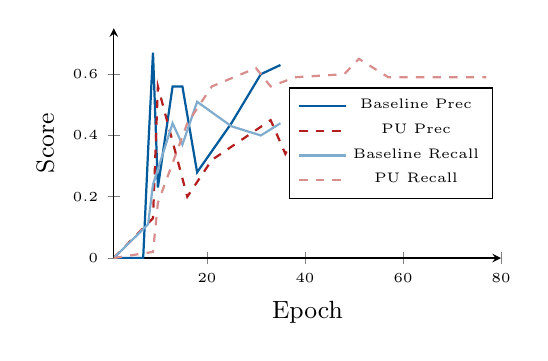
\begin{tikzpicture}
        \begin{axis}[
            width=6.5cm, height=4.5cm,
            xlabel={\small Epoch},
            ylabel={\small Score},
            xmin=1, xmax=80,
            ymin=0, ymax=0.75,
            tick label style={font=\tiny},
            axis lines=left,
            legend style={font=\tiny, at={(0.98,0.5)}, anchor=east},
          ]
          % Baseline precision
          \addplot[color=accent, thick] coordinates {
            (1,0)(7,0)(8,0.35)(9,0.67)(10,0.23)(13,0.56)(15,0.56)
            (18,0.28)(25,0.44)(31,0.60)(35,0.63)
          };
          % PU-loss precision
          \addplot[color=bad, thick, dashed] coordinates {
            (1,0)(9,0.13)(10,0.56)(16,0.20)(21,0.32)
            (33,0.45)(36,0.34)(38,0.40)(48,0.36)(51,0.36)(57,0.41)(77,0.41)
          };
          % Baseline recall
          \addplot[color=accent!50, thick] coordinates {
            (1,0)(8,0.11)(9,0.24)(13,0.44)(15,0.37)
            (18,0.51)(25,0.43)(31,0.40)(35,0.44)
          };
          % PU-loss recall
          \addplot[color=bad!50, thick, dashed] coordinates {
            (1,0)(9,0.02)(10,0.18)(16,0.44)(21,0.56)
            (30,0.62)(33,0.56)(38,0.59)(48,0.60)(51,0.65)(57,0.59)(77,0.59)
          };
          \legend{Baseline Prec, PU Prec, Baseline Recall, PU Recall}
        \end{axis}
      \end{tikzpicture}
    \end{column}
    \begin{column}{0.46\textwidth}
      \vspace{2pt}
      \textbf{Key observations:}
      \begin{itemize}\small
        \item Baseline converges to \textbf{high precision / moderate recall} — conservative detector
        \item PU Loss achieves \textbf{higher recall at comparable precision} — better coverage of true positives
        \item PU Loss recall steadily climbs past epoch 40; baseline recall plateaus at $\sim$0.49
        \item The soft-sampling term in PU Loss effectively suppresses false negatives from unlabeled positives
      \end{itemize}

      \vspace{6pt}
      \begin{block}{\small Clinical relevance}
        \scriptsize Higher recall reduces missed detections — critical for a screening workflow where false negatives carry higher clinical cost than false positives.
      \end{block}
    \end{column}
  \end{columns}
\end{frame}

% ── SLIDE CMP-6 — Conclusions ─────────────────────────────────────────────────
\begin{frame}{Conclusions: PU Loss After HPO}
  \begin{columns}[T]
    \begin{column}{0.50\textwidth}
      \textbf{Before HPO (earlier investigation):}
      \begin{itemize}\small
        \item PU Loss degraded mAP vs baseline
        \item Gradient re-weighting interacted poorly with high LR and low weight decay
        \item Inconsistent convergence
      \end{itemize}

      \vspace{8pt}
      \textbf{After HPO (current runs):}
      \begin{itemize}\small
        \item PU Loss outperforms baseline on all detection metrics
        \item $10\times$ higher weight decay ($9.7 \times 10^{-3}$) stabilises PU gradient re-weighting
        \item Longer convergence (epoch 57 vs 15) — patience=20 essential
        \item Slice-AP@50 also improved
      \end{itemize}
    \end{column}
    \begin{column}{0.46\textwidth}
      \vspace{2pt}
      \begin{block}{\small Overall progression}
        \small
        \begin{tabular}{lcc}
          \toprule
          Stage & AP@50 & Note \\
          \midrule
          Pre-fix baseline     & 0.40 & loss norm bug \\
          Post-fix baseline    & 0.45 & HPO default config \\
          HPO best trial       & 0.58 & 50-ep trial \\
          \rowcolor{rowhl}
          Baseline (full, HPO) & 0.45 & 35 ep, early stop \\
          \rowcolor{rowhl}
          \textbf{PU Loss (full, HPO)} & \textbf{0.56} & \textbf{77 ep} \\
          \bottomrule
        \end{tabular}
      \end{block}

      \vspace{6pt}
      \textbf{Next:}
      \begin{itemize}\small
        \item Extend PU Loss run to 150 epochs (patience=30) — learning curve still ascending at epoch 77
        \item Evaluate on held-out test set
        \item Pseudo-labeling iteration using PU Loss checkpoint
      \end{itemize}
    \end{column}
  \end{columns}
\end{frame}

\end{document}
